\documentclass[UTF8]{ctexart}
\usepackage{geometry}
\geometry{margin=1.5cm, vmargin={0pt,1cm}}
\setlength{\topmargin}{-1cm}
\setlength{\paperheight}{29.7cm}
\setlength{\textheight}{25.3cm}

% useful packages.
\usepackage{amsfonts}
\usepackage{amsmath}
\usepackage{amssymb}
\usepackage{amsthm}
\usepackage{enumerate}
\usepackage{graphicx}
\usepackage{multicol}
\usepackage{fancyhdr}
\usepackage{layout}
\usepackage{float, caption}
\usepackage{xcolor}
\usepackage{listings}
\usepackage{tikz}
\usepackage{graphicx}
\usepackage{subcaption}  % 使用subcaption宏包

% 自定义配色方案,尽量模仿 VS Code 的高亮效果
\definecolor{codegreen}{rgb}{0,0.6,0}
\definecolor{codeblue}{rgb}{0,0,0.9}
\definecolor{codepurple}{rgb}{0.58,0,0.82}
\definecolor{codered}{rgb}{0.8,0,0}
\definecolor{backcolor}{rgb}{0.95,0.95,0.95}

% lstlisting 的风格设置
\lstdefinestyle{vscode}{
	backgroundcolor=\color{backcolor},   % 背景颜色
	commentstyle=\color{codegreen},     % 注释颜色
	keywordstyle=\color{codeblue}\bfseries, % 关键字颜色
	numberstyle=\tiny\color{gray},      % 行号颜色
	stringstyle=\color{codered},        % 字符串颜色
	basicstyle=\ttfamily\footnotesize,  % 基本字体
	breakatwhitespace=false,            % 仅在空格处断行
	breaklines=true,                    % 自动换行
	captionpos=b,                       % 标题位置(bottom)
	keepspaces=true,                    % 保持空格
	numbers=left,                       % 显示行号
	numbersep=5pt,                      % 行号与代码间的间隔
	rulecolor=\color{black},            % 框线颜色
	showspaces=false,                   % 不显示空格符号
	showstringspaces=false,             % 不显示字符串中的空格
	showtabs=false,                     % 不显示制表符
	frame=single,                       % 外框
	tabsize=4,                          % 制表符宽度
	escapeinside={(*@}{@*)},            % 特殊字符转义
	morekeywords={*,...}                % 添加更多自定义关键字
}
\lstset{style=vscode}

% some common command
\newcommand{\dif}{\mathrm{d}}
\newcommand{\avg}[1]{\left\langle #1 \right\rangle}
\newcommand{\difFrac}[2]{\frac{\dif #1}{\dif #2}}
\newcommand{\pdfFrac}[2]{\frac{\partial #1}{\partial #2}}
\newcommand{\OFL}{\mathrm{OFL}}
\newcommand{\UFL}{\mathrm{UFL}}
\newcommand{\fl}{\mathrm{fl}}
\newcommand{\op}{\odot}
\newcommand{\Eabs}{E_{\mathrm{abs}}}
\newcommand{\Erel}{E_{\mathrm{rel}}}

\begin{document}
	
	\pagestyle{fancy}
	\fancyhead{}
	\lhead{高凌溪, 3210105373}
	\chead{2024DS编程作业报告}
	\rhead{\today}
	\begin{abstract}
		题目的运行结果和分析
	\end{abstract}
	\section{A 用pp样条拟合函数}
		\begin{figure}[H]
		\centering
		\begin{subfigure}[b]{0.45\textwidth}
			\centering
			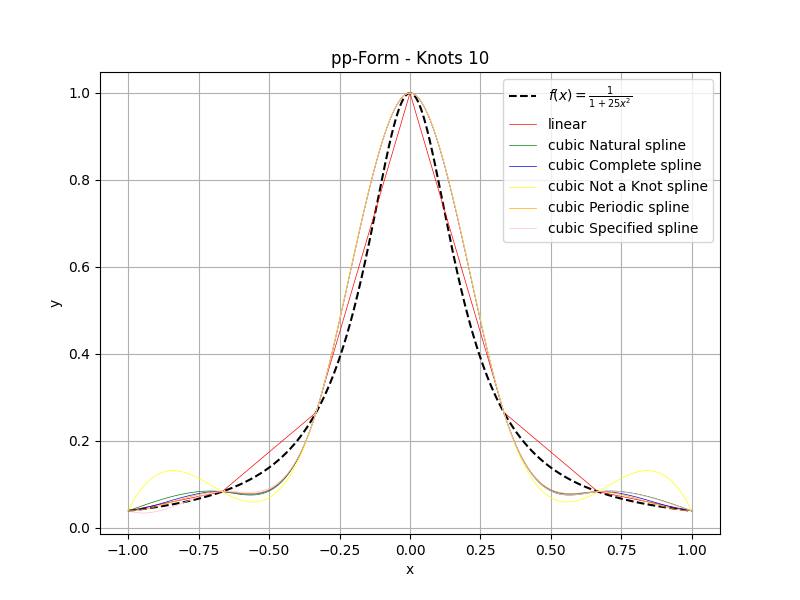
\includegraphics[width=\textwidth]{../figure/A_1.png}
			\caption{6 knots}
			\label{fig:image1}
		\end{subfigure}
		\hspace{0.5cm}  % 控制两张图片之间的间距
		\begin{subfigure}[b]{0.45\textwidth}
			\centering
			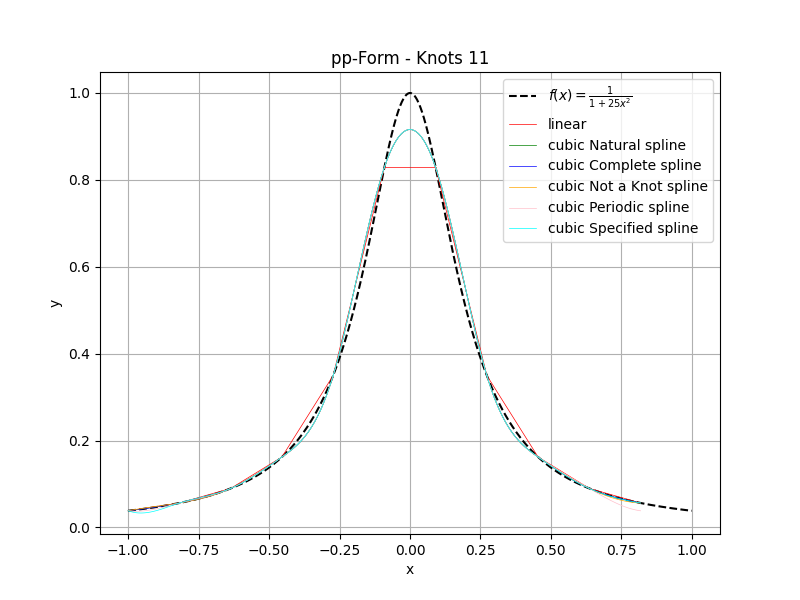
\includegraphics[width=\textwidth]{../figure/A_2.png}
			\caption{11 knots}
			\label{fig:image2}
		\end{subfigure}
		\caption{pp样条拟合函数}
		\label{fig:two_images}
	\end{figure}
	
	\begin{figure}[H]
		\centering
		\begin{subfigure}[b]{0.45\textwidth}
			\centering
			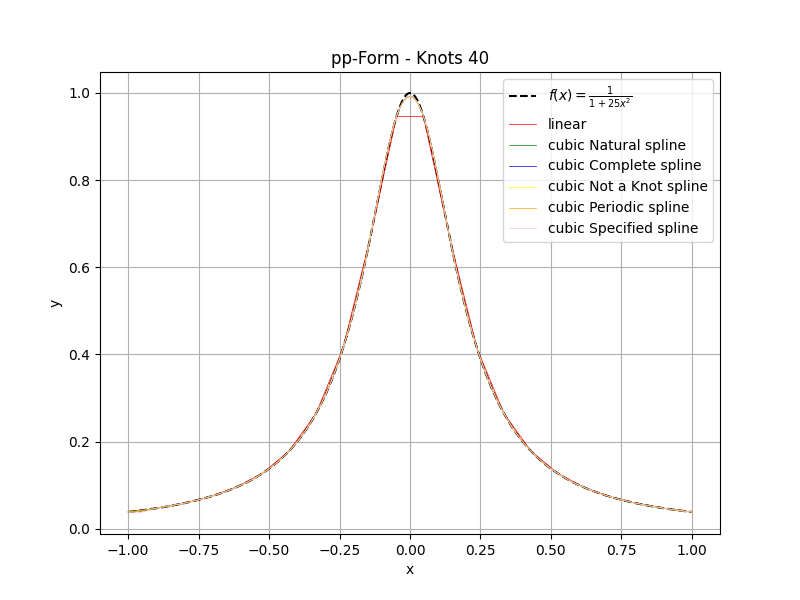
\includegraphics[width=\textwidth]{../figure/A_3.png}
			\caption{21 knots}
			\label{fig:image1}
		\end{subfigure}
		\hspace{0.5cm}  % 控制两张图片之间的间距
		\begin{subfigure}[b]{0.45\textwidth}
			\centering
			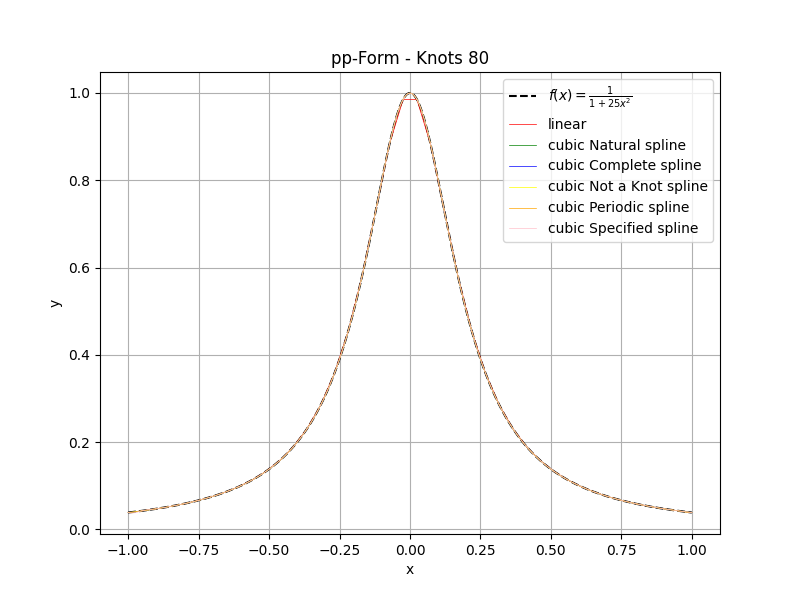
\includegraphics[width=\textwidth]{../figure/A_4.png}
			\caption{41 knots}
			\label{fig:image2}
		\end{subfigure}
		\caption{pp样条拟合函数}
		\label{fig:two_images}
	\end{figure}
	
	\begin{figure}[H]
		\centering
		\begin{subfigure}[b]{0.45\textwidth}
			\centering
			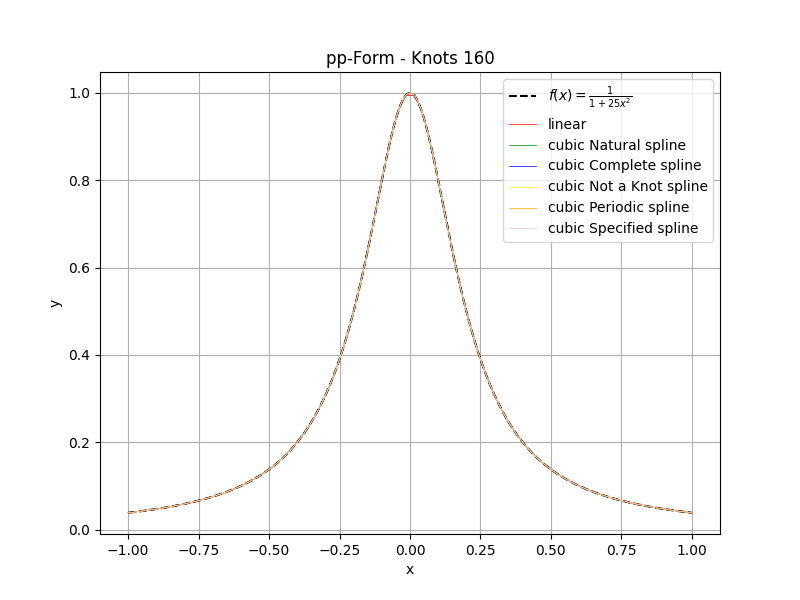
\includegraphics[width=\textwidth]{../figure/A_5.png}
			\caption{81 knots}
			\label{fig:image1}
		\end{subfigure}
	\end{figure}
	几种情况下在区间中点的误差为
	\begin{table}[H]
		\centering
		\begin{tabular}{|c|c|c|c|c|c|c|}
			\hline
			 & linear & natural & complete & not-a-knot & periodic & specified \\
			\hline
			knots 6 & 0.042189 & 0.131401 & 0.129445 & 0.177149 & 0.135823 & 0.133095 \\
			\hline
			knots 11 & 0.0417277 & 0.047166 & 0.0471638 & 0.0472169 & 0.0473469 & 0.0471672 \\
			\hline
			3knots 21 & 0.0135534 & 0.0044802 & 0.0044802 & 0.0044802 & 0.0044802 & 0.00448023 \\
			\hline
			knots 41 & 0.00367977 & 0.000139672 & 0.000139672 & 0.000139672 & 0.000553506 & 0.000557674 \\
			\hline
			knots 81 & 0.000950222 & 6.43681e-06 & 6.41586e-06 & 6.41586e-06 & 0.000270492 & 0.000275263 \\
			\hline
		\end{tabular}
		\caption{不同节点和样条拟合的最大误差}
	\end{table}
	用$N$表示节点数目。对于$S_3^2$最大误差关于节点的最大误差大约是$10^{-log_2N}$,对于线性样条,$N$比较小的时候比较难判断,但是$N$很大的时候,最大误差大约是$10^{-log_2N+1}$
	
	
	\section{C 用b样条拟合$\frac{1}{1+x^2}$}
	使用五种不同边界条件的$S_3^2$ B样条和线性样条拟合,结果如下
	\begin{figure}[H]
		\centering
		\begin{subfigure}[b]{0.45\textwidth}
			\centering
			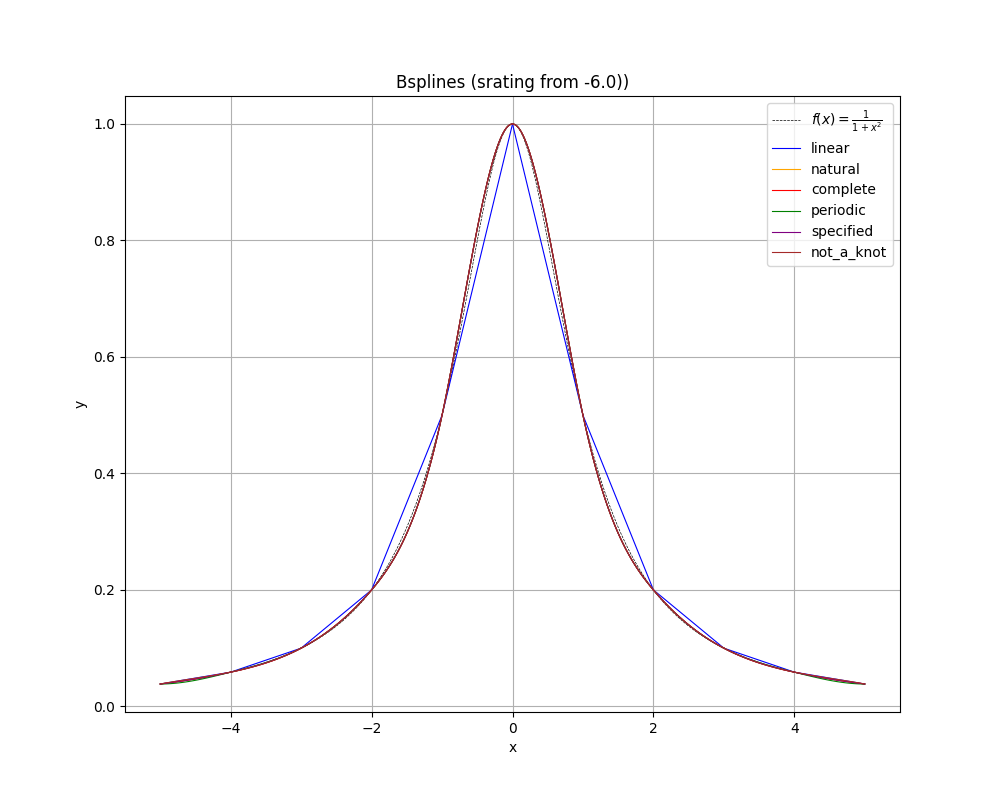
\includegraphics[width=\textwidth]{../figure/C_1.png}
			\caption{$t_i=-6+i$}
			\label{fig:image1}
		\end{subfigure}
		\hspace{0.5cm}  % 控制两张图片之间的间距
		\begin{subfigure}[b]{0.45\textwidth}
			\centering
			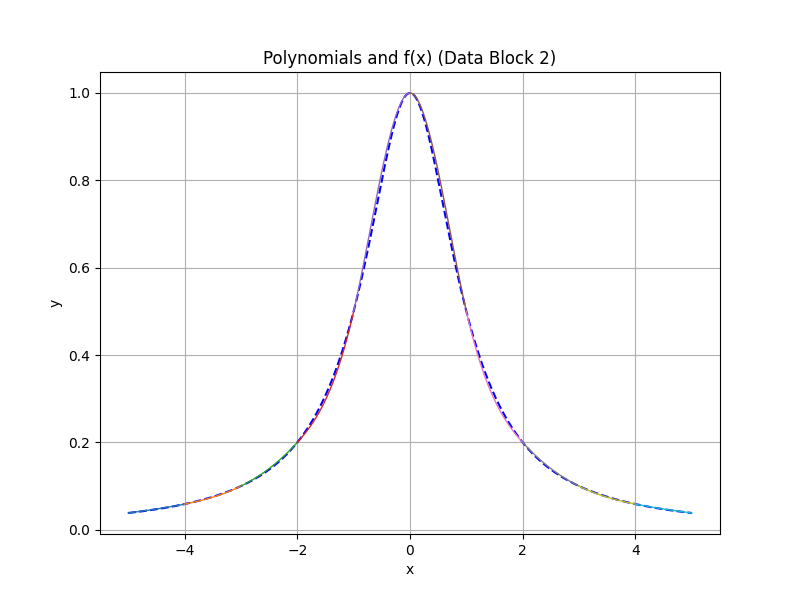
\includegraphics[width=\textwidth]{../figure/C_2.png}
			\caption{$t_i=-5.5+i$}
			\label{fig:image2}
		\end{subfigure}
		\caption{B样条拟合函数}
		\label{fig:two_images}
	\end{figure}
	\begin{figure}[H]
		\centering
		\begin{subfigure}[b]{0.45\textwidth}
			\centering
			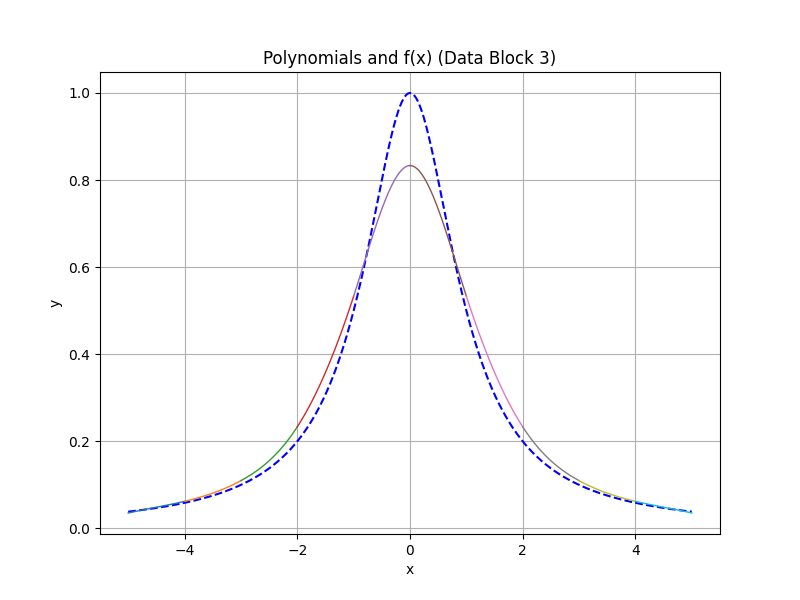
\includegraphics[width=\textwidth]{../figure/C_3.png}
			\caption{$Theorem 3.58$}
			\label{$S_2^1$样条拟合函数}
		\end{subfigure}
	\end{figure}
	我们可以看出来,对于一个轴对称的函数来说,要想让最大误差尽可能地小,应该取奇数个节点,并且在对称轴上取一个节点。
	\section{D 特定节点上的误差}
	两种取节点的方式下,对不同样条得到的误差如下:
\begin{table}[H]
	\centering
	\begin{tabular}{|c|c|c|c|c|c|c|c|}
		\hline
		\textbf{knots} & -3.5 & -3 & -0.5 & 0 & 0.5 & 3 & 3.5 \\
		\hline
		\textbf{linear} & -0.00394007 & -1.38778e-17 & 0.05 & 0 & 0.05 & -2.77556e-17 & -0.00394007 \\
		\hline
		\textbf{quadratic} & 1.249e-16 & -0.00141838 & 0 & 0.1202380 & 0 & -0.00141838 &  1.249e-16  \\
		\hline
		\textbf{cubic\_natural} & 0.000789971 & 1.38778e-16 & -0.0205306 & 0 & -0.0205306 & -8.60423e-16 & 0.000789971 \\
		\hline
	\end{tabular}
	\caption{三种B样条在给定节点上的误差}
\end{table}
	这里$-3,\ 3,\ 0$正好是一阶和三阶B样条的节点,因此误差应该是0,而在$3,\ -3$处数据很接近机器误差是因为B样条是又基函数和系数决定的,系数是通过求解线性方程组得到,而接近0的浮点数在计算机里会有catastrophic cancellation的现象,因此误差会在机器误差左右。
	
	综合来看,如果用最大误差来作为衡量标准,$S_2^1$样条的效果不如$S_3^2$,对于不同边界条件的$S_3^2$样条的误差,可以在终端输出的信息中找到,这里就不再列出。
\section{E 曲线拟合}
对于曲线拟合的结果,由于图片太多,这里只放几张比较有代表性的,所有的结果都可以在figure文件夹找到。\\
对平面曲线的cumulate\_chordal参数,分别用pp样条和B样条拟合,用来验证两种样条得到的结果相同;由于B样条需要额外取节点,因此对于均匀节点作为参数,只用了pp样条拟合,把这三种拟合的结果放在一起对比,能够看出如果节点一致B样条和pp样条得到的结果是相同的,这正好对应了定理3.7.\\
拟合心形线,因为是闭合曲线,所以边界条件选择periodic
	\begin{figure}[H]
	\centering
	\begin{subfigure}[b]{0.45\textwidth}
		\centering
		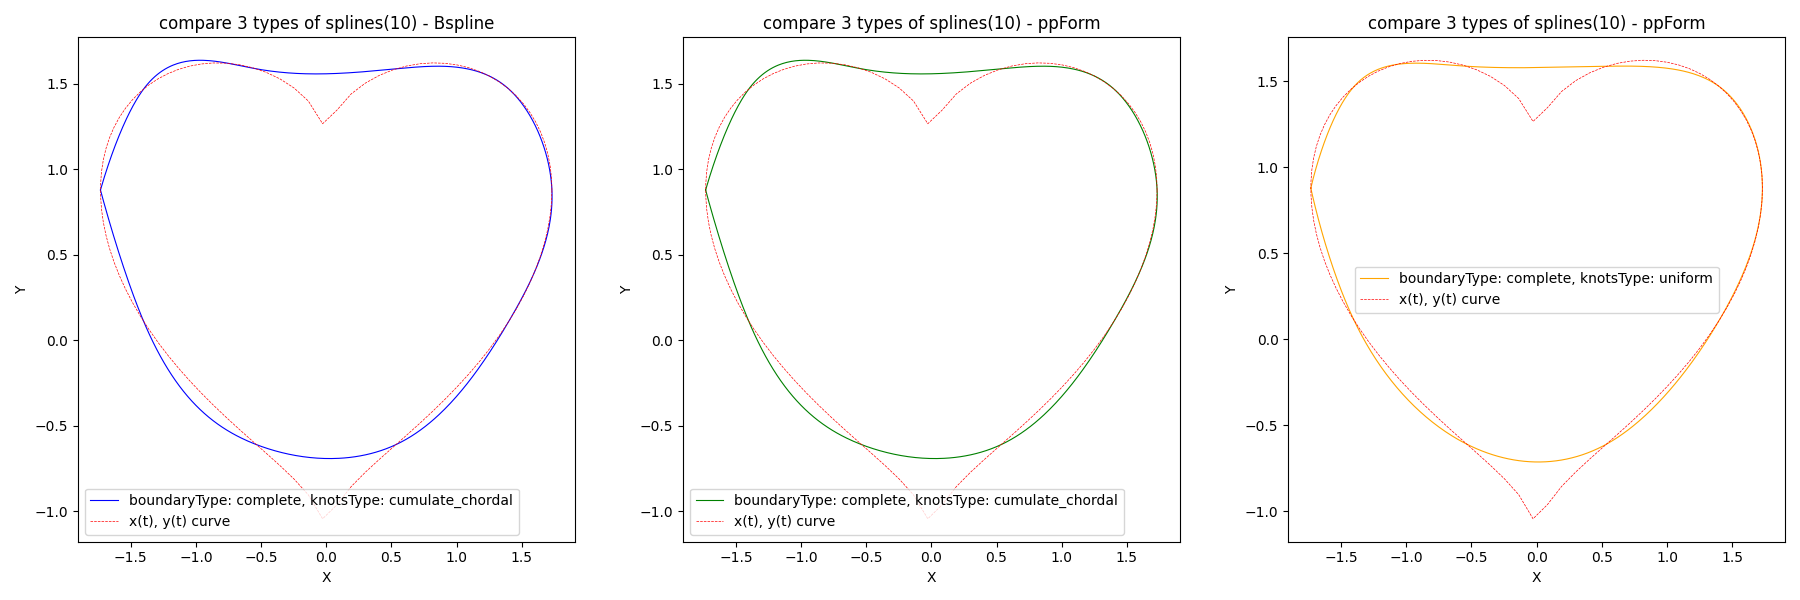
\includegraphics[width=\textwidth]{../figure/E_curve1.json_1.png}
		\caption{10 knots}
		\label{fig:image1}
	\end{subfigure}
	\hspace{0.5cm}  % 控制两张图片之间的间距
	\begin{subfigure}[b]{0.45\textwidth}
		\centering
		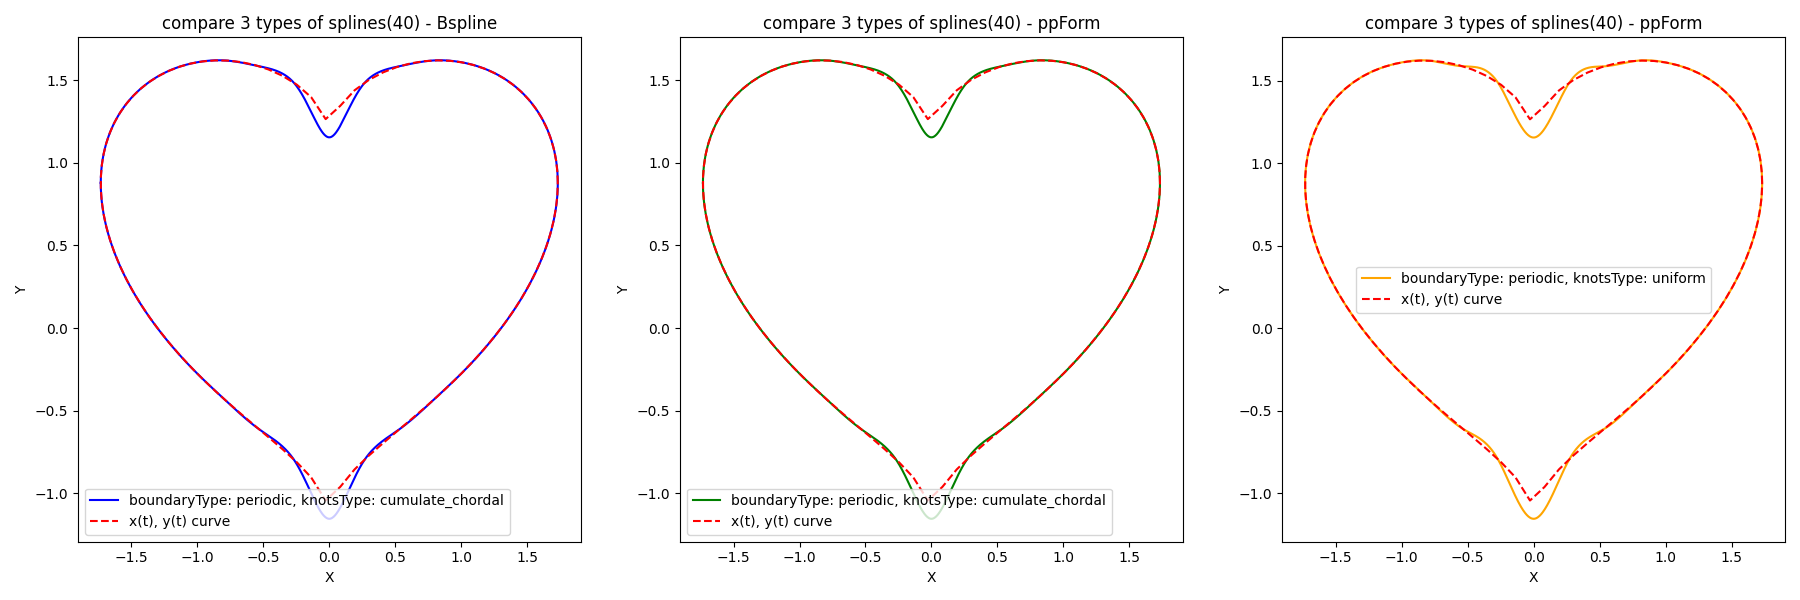
\includegraphics[width=\textwidth]{../figure/E_curve1.json_6.png}
		\caption{40 knots}
		\label{fig:image2}
	\end{subfigure}
	\caption{拟合心形函数}
	\label{fig:two_images}
\end{figure}
\begin{figure}[H]
	\centering
	\begin{subfigure}[b]{0.45\textwidth}
		\centering
		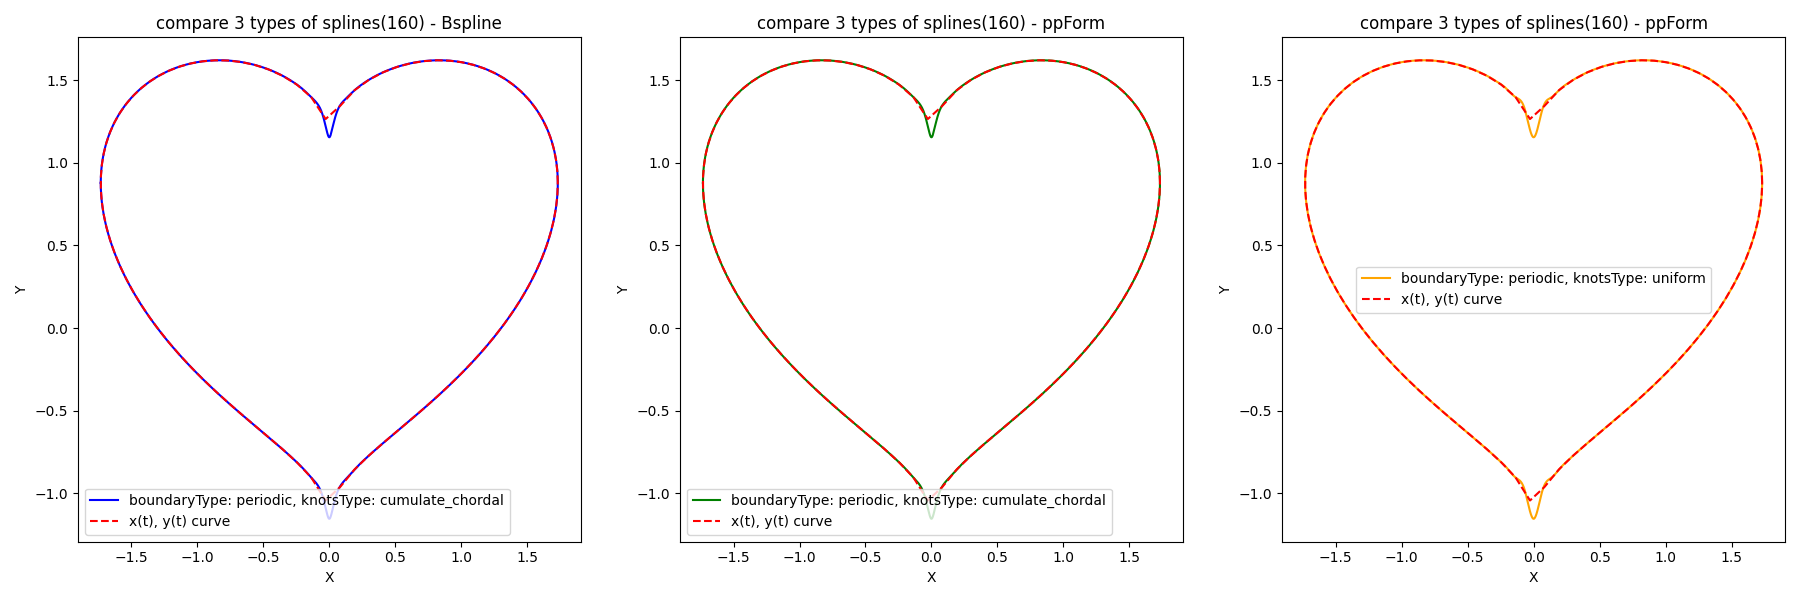
\includegraphics[width=\textwidth]{../figure/E_curve1.json_10.png}
		\caption{160 knots}
		\label{fig:image1}
	\end{subfigure}
\end{figure}
我们能发现,在$x=0$的时候,拟合效果是最差的,猜测这是由于心形线本来在这些点并不可导,而$S_3^2$本身有二阶正则性。\\
拟合螺旋形,选择了natural边界条件
	\begin{figure}[H]
	\centering
	\begin{subfigure}[b]{0.45\textwidth}
		\centering
		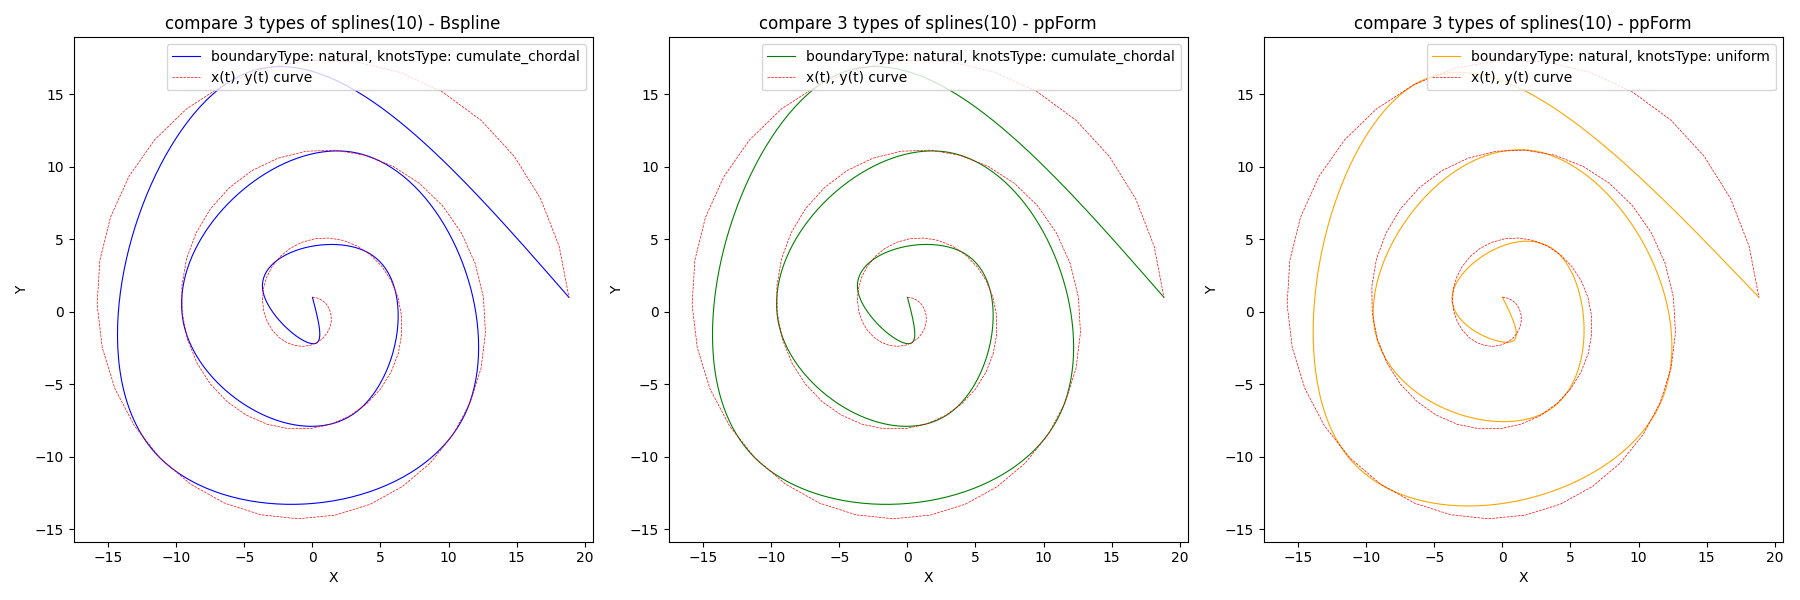
\includegraphics[width=\textwidth]{../figure/E_curve2.json_3.png}
		\caption{10 knots}
		\label{fig:image1}
	\end{subfigure}
	\hspace{0.5cm}  % 控制两张图片之间的间距
	\begin{subfigure}[b]{0.45\textwidth}
		\centering
		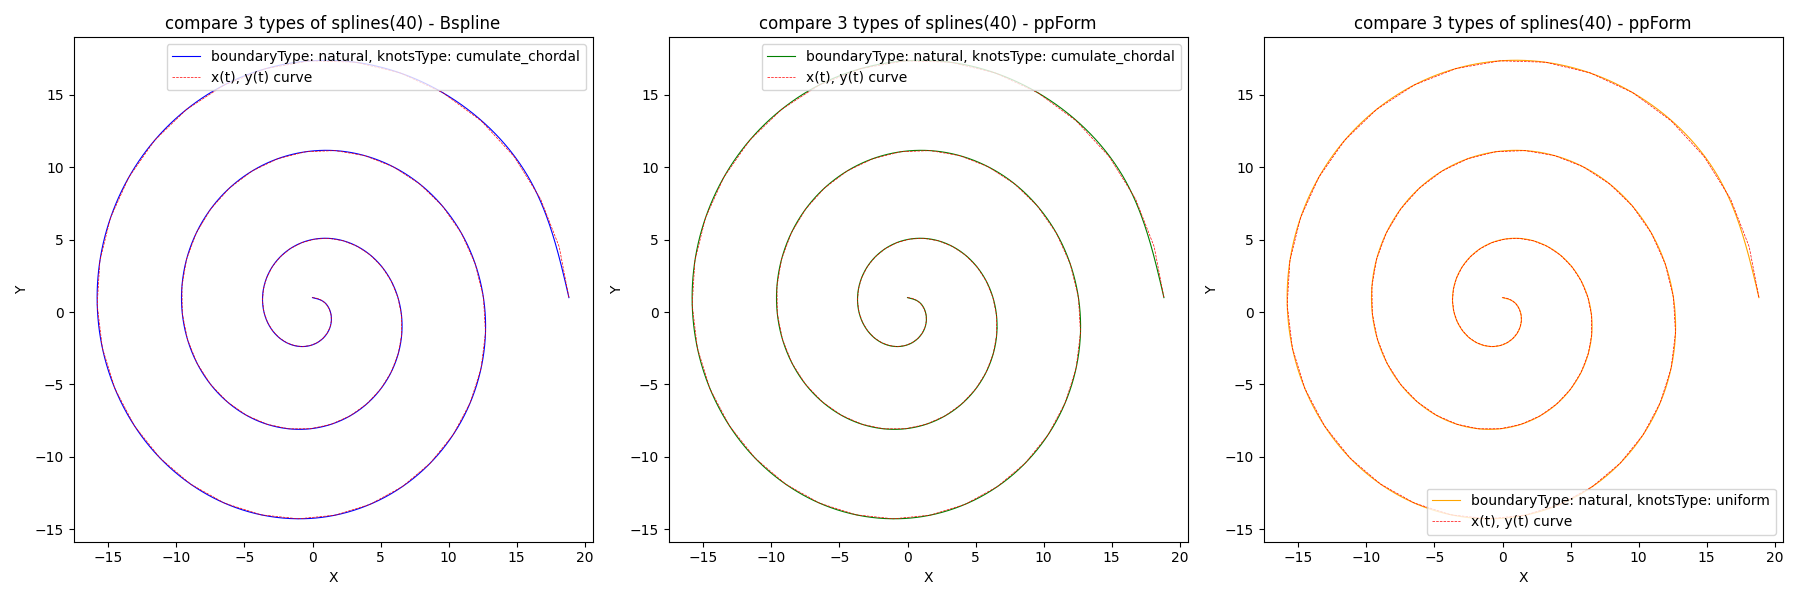
\includegraphics[width=\textwidth]{../figure/E_curve2.json_7.png}
		\caption{40 knots}
		\label{fig:image2}
	\end{subfigure}
	\caption{拟合螺旋线}
	\label{fig:two_images}
\end{figure}
\begin{figure}[H]
	\centering
	\begin{subfigure}[b]{0.45\textwidth}
		\centering
		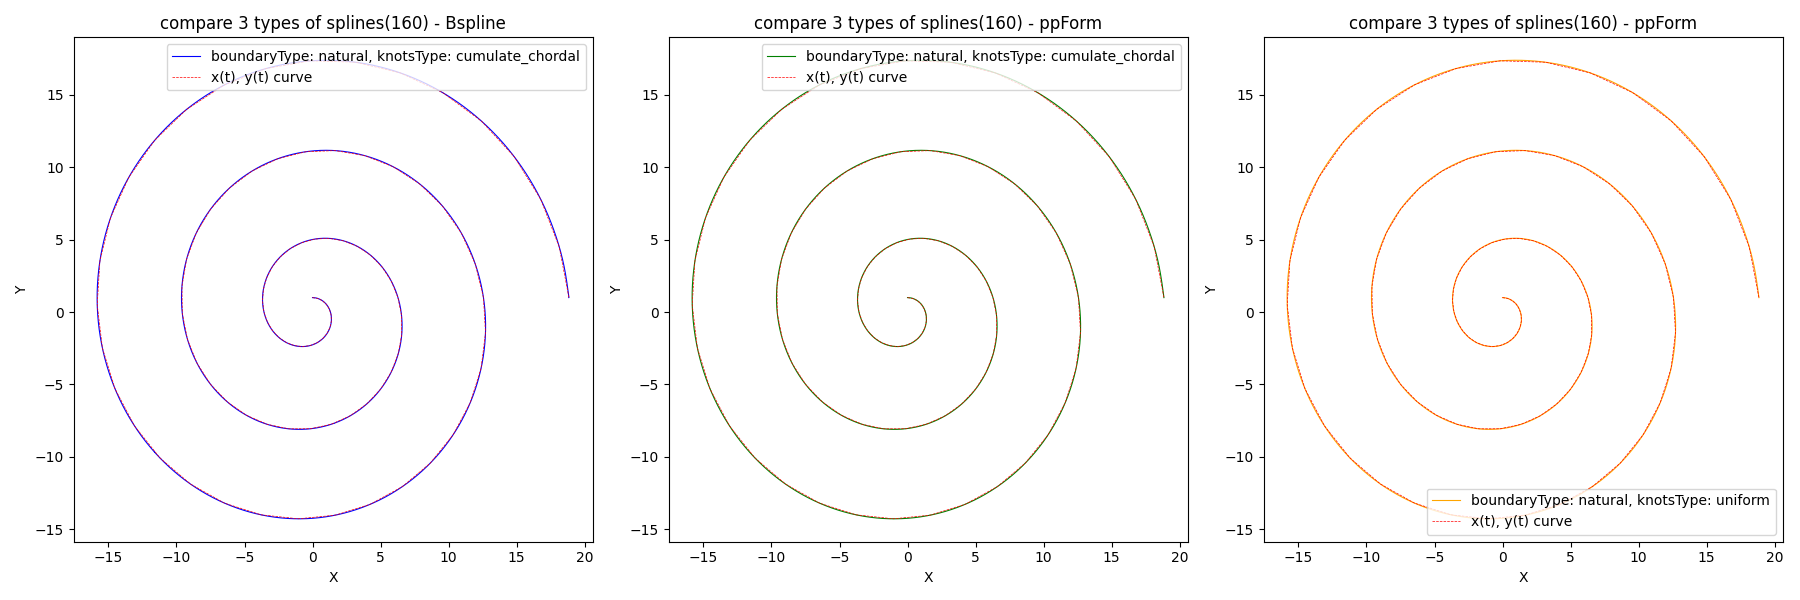
\includegraphics[width=\textwidth]{../figure/E_curve2.json_11.png}
		\caption{160 knots}
		\label{fig:image1}
	\end{subfigure}
\end{figure}
拟合球面曲线,选择了complete边界条件
\begin{figure}[H]
	\centering
	\begin{subfigure}[b]{0.45\textwidth}
		\centering
		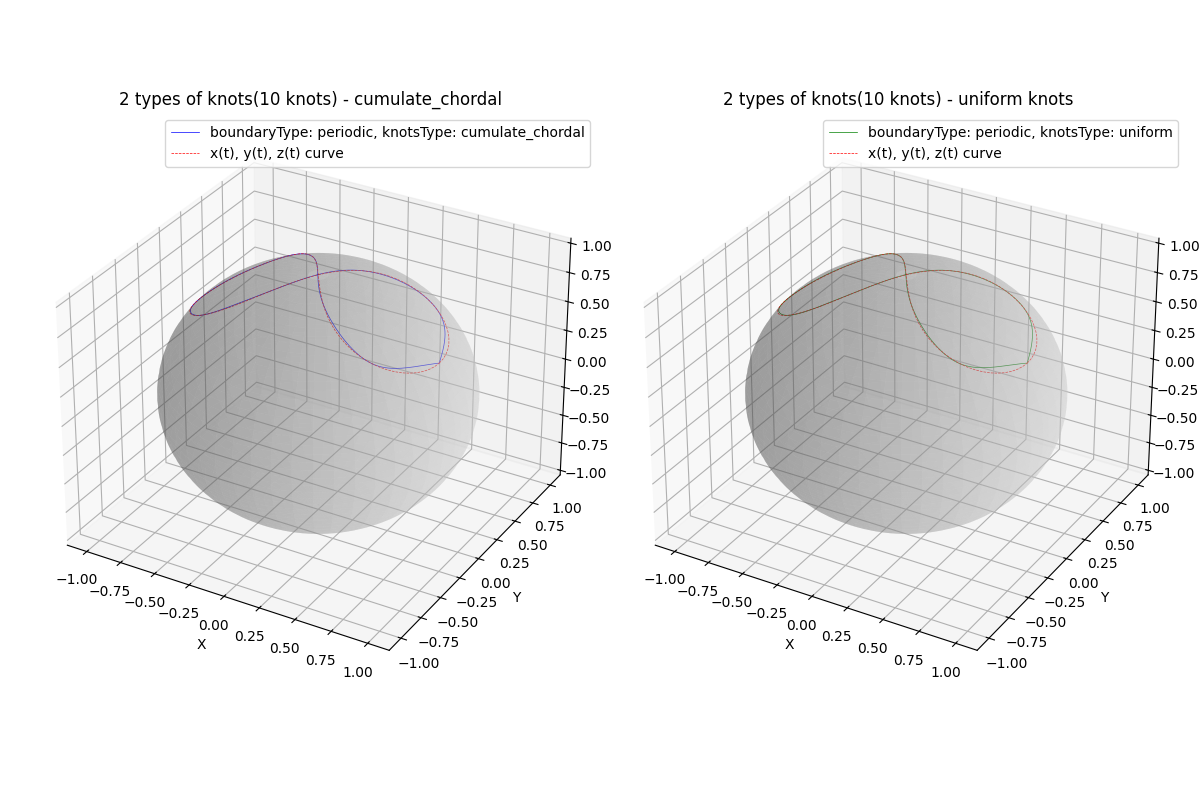
\includegraphics[width=\textwidth]{../figure/plot_1.png}
		\caption{10 knots}
		\label{fig:image1}
	\end{subfigure}
	\hspace{0.5cm}  % 控制两张图片之间的间距
	\begin{subfigure}[b]{0.45\textwidth}
		\centering
		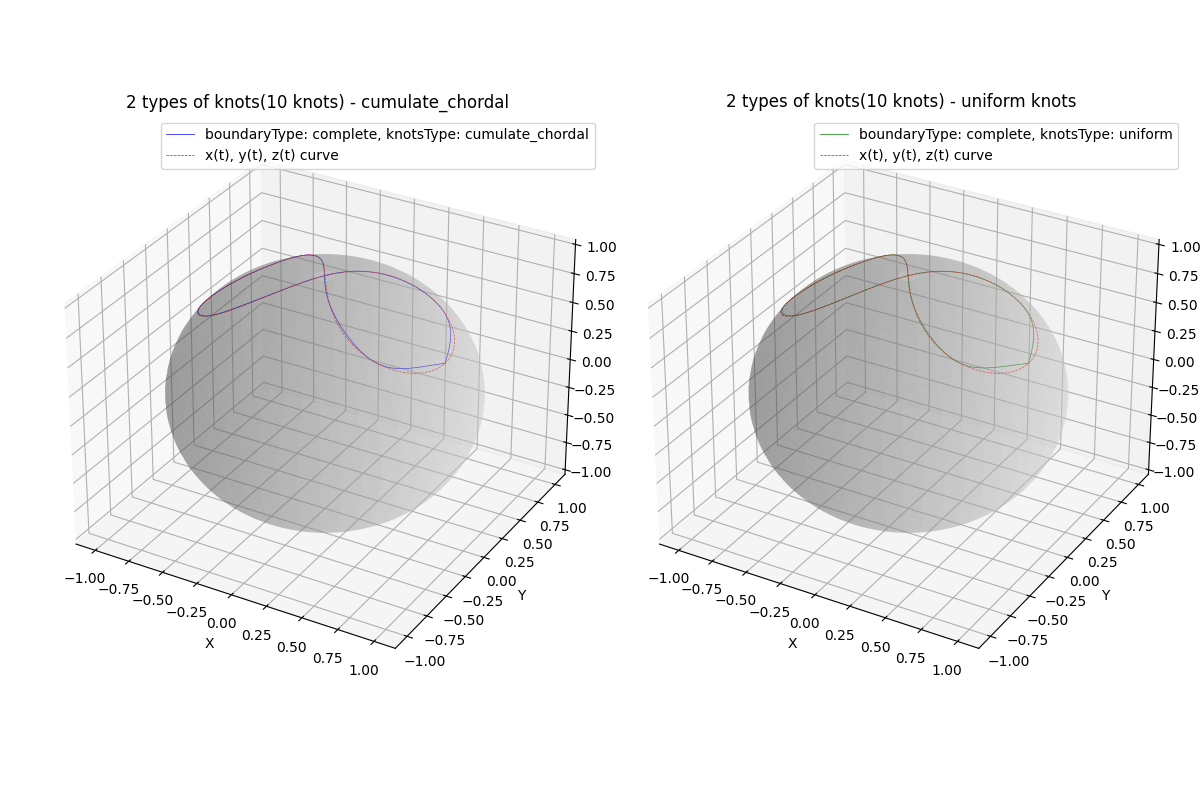
\includegraphics[width=\textwidth]{../figure/plot_3.png}
		\caption{40 knots}
		\label{fig:image2}
	\end{subfigure}
	\caption{拟合球面曲线}  % 删除了多余的右括号
	\label{fig:two_images}
\end{figure}

\begin{figure}[H]
	\centering
	\begin{subfigure}[b]{0.45\textwidth}
		\centering
		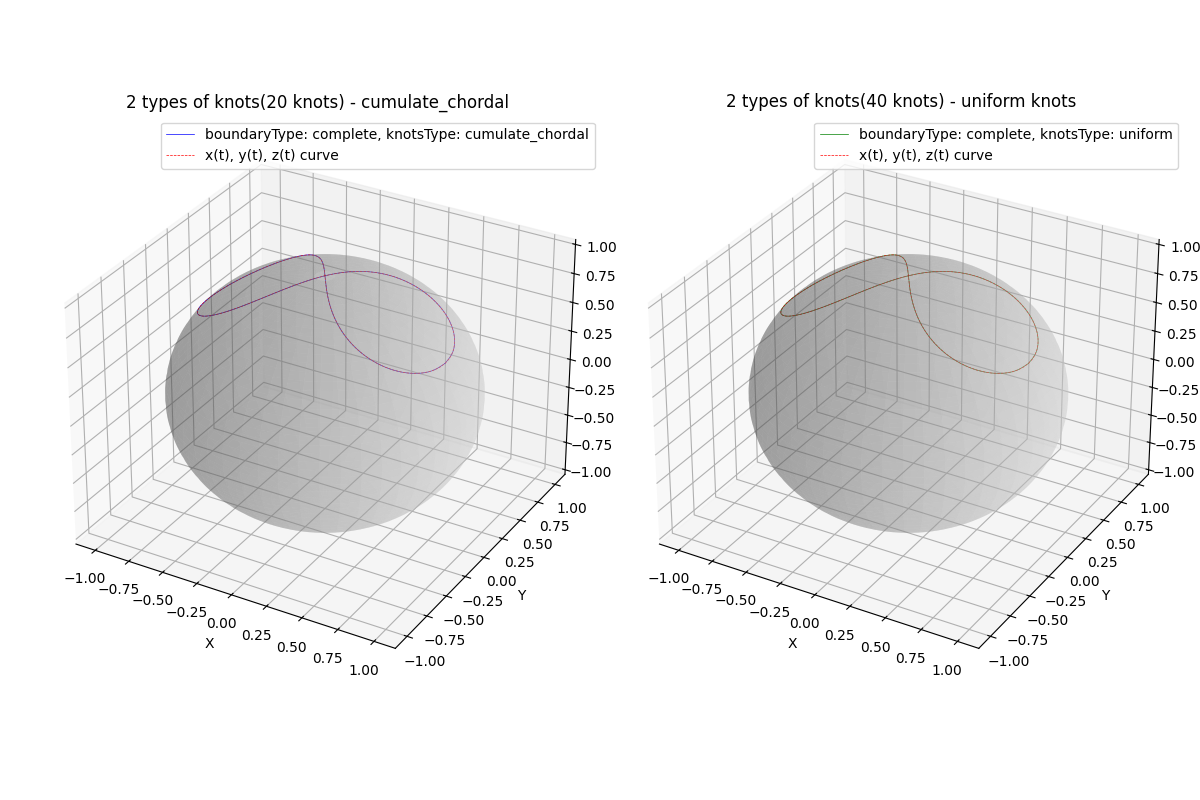
\includegraphics[width=\textwidth]{../figure/plot_7.png}
		\caption{10 knots}
		\label{fig:image1}
	\end{subfigure}
	\hspace{0.5cm}  % 控制两张图片之间的间距
	\begin{subfigure}[b]{0.45\textwidth}
		\centering
		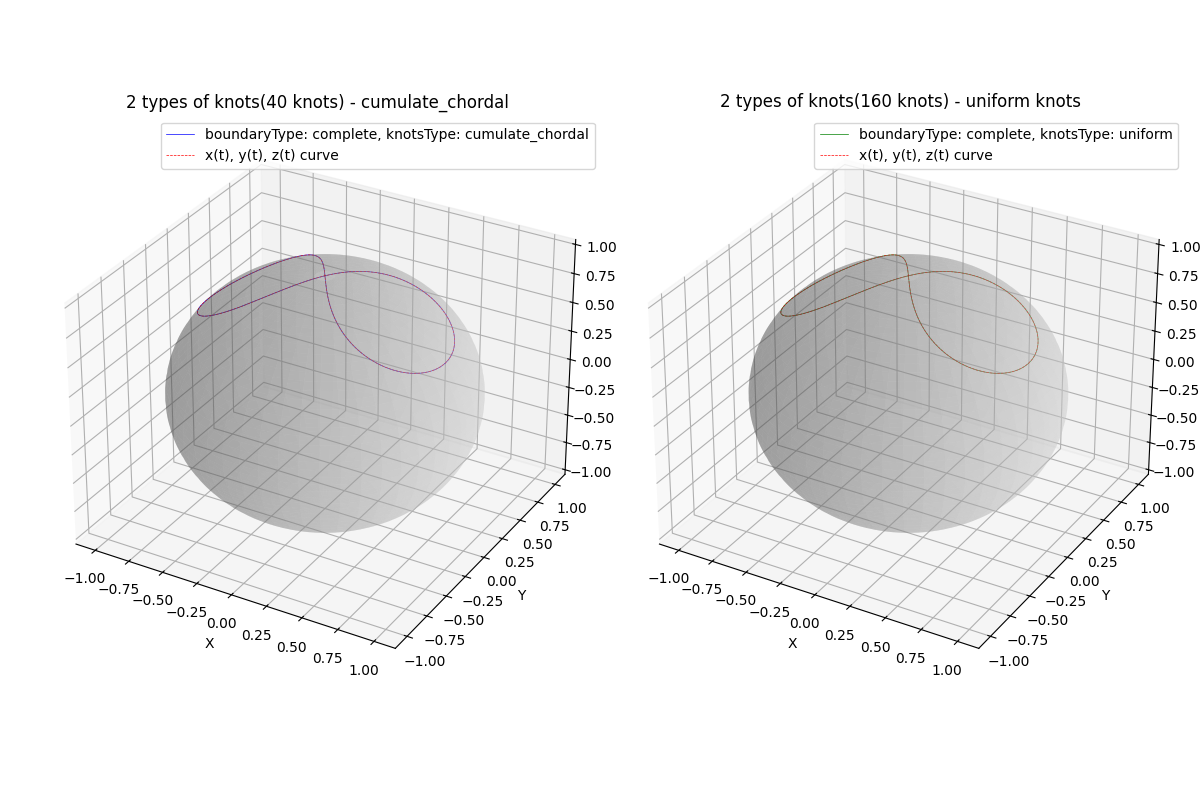
\includegraphics[width=\textwidth]{../figure/plot_11.png}
		\caption{40 knots}
		\label{fig:image2}
	\end{subfigure}
	\caption{拟合球面曲线} 
	\label{fig:two_images}
\end{figure}
当取的节点很少的时候,两种曲线参数差别会有一点,尤其是对螺旋线选择了periodic边界条件,如果只用极坐标下的均匀节点,能看出拟合的样条曲线在第一个节点处非常“尖锐”。这里推测均匀节点得到的样条曲线可能比cumulative chordal lengths节点更容易自交。
%%------------------------------------------------------------------------
\section{F $(t-x)_{+}^n$的差商表}
根据题目的意思,对$t$做插商,则差商表的每个元素是关于$x$的函数,$n=1$时,节点选择$0.0,\  1.0,\  2.0$,结果如下:\\
% 第一行:一张图片
\noindent % 确保左对齐
\begin{minipage}{0.3\textwidth}
	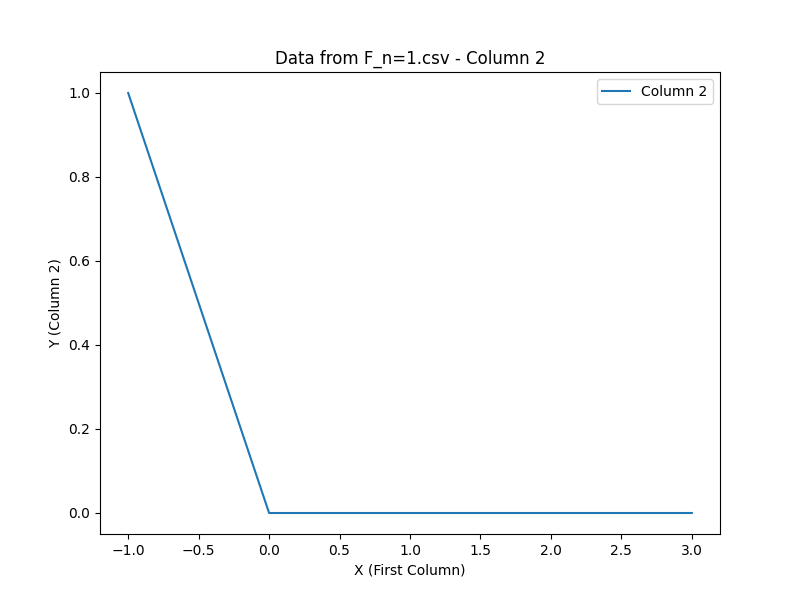
\includegraphics[width=\linewidth]{../figure/F_n=1.csv_Column_2.png} % 替换为你的图片路径
\end{minipage}

\vspace{0.5em} % 添加垂直间距

% 第二行:两张图片
\noindent % 确保左对齐
\begin{minipage}{0.3\textwidth}
	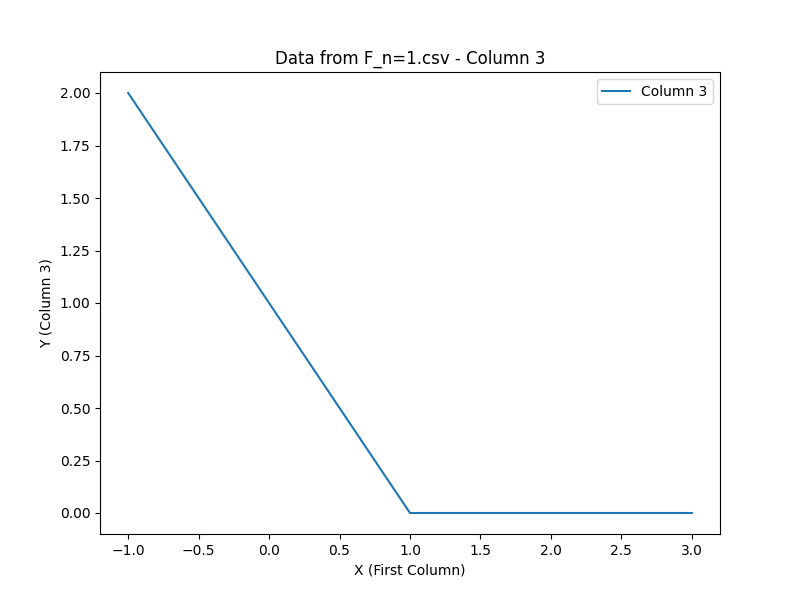
\includegraphics[width=\linewidth]{../figure/F_n=1.csv_Column_3.png} % 替换为你的图片路径
\end{minipage}
\hspace{1em} % 添加水平间距
\begin{minipage}{0.3\textwidth}
	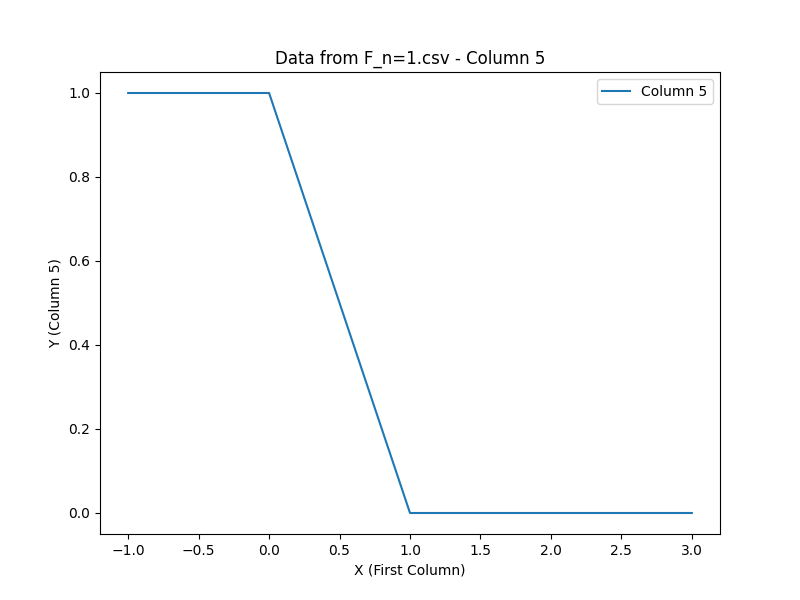
\includegraphics[width=\linewidth]{../figure/F_n=1.csv_Column_5.png} % 替换为你的图片路径
\end{minipage}

\vspace{0.5em} % 添加垂直间距

% 第三行:三张图片
\noindent % 确保左对齐
\begin{minipage}{0.3\textwidth}
	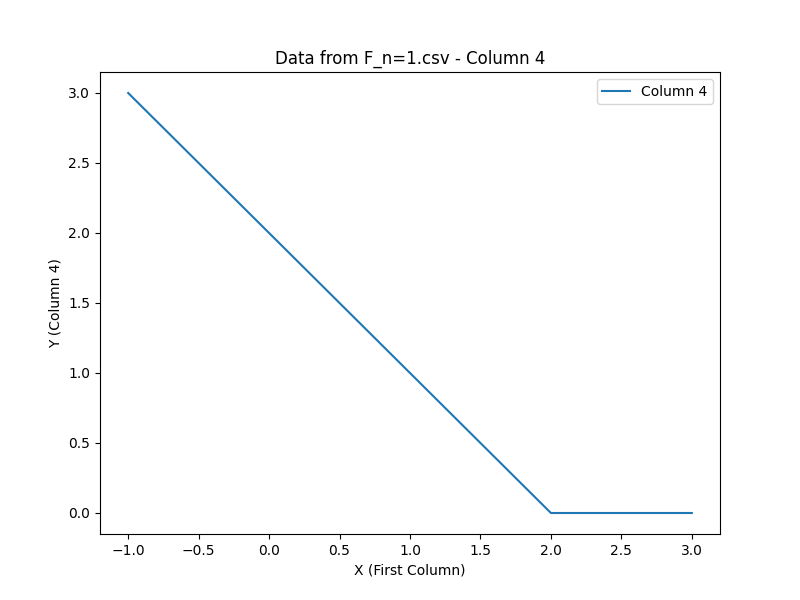
\includegraphics[width=\linewidth]{../figure/F_n=1.csv_Column_4.png} % 替换为你的图片路径
\end{minipage}
\hspace{1em} % 添加水平间距
\begin{minipage}{0.3\textwidth}
	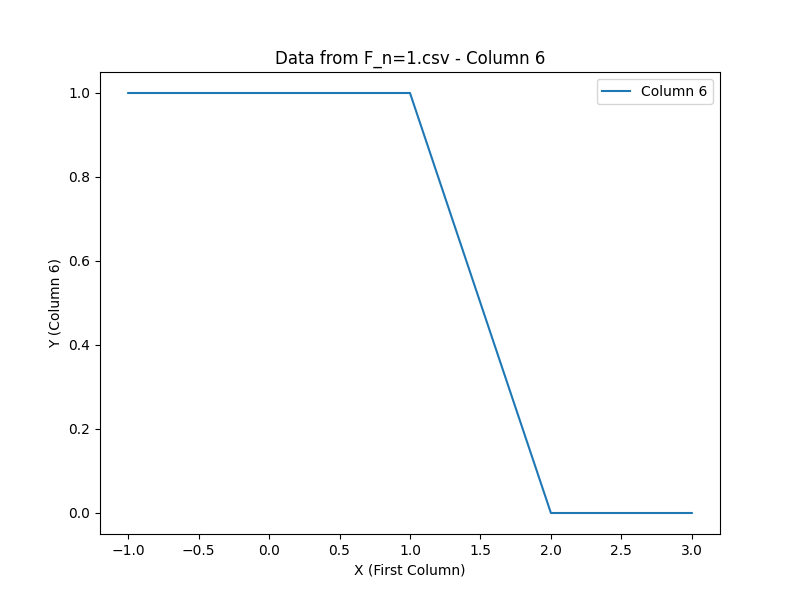
\includegraphics[width=\linewidth]{../figure/F_n=1.csv_Column_6.png} % 替换为你的图片路径
\end{minipage}
\hspace{1em} % 添加水平间距
\begin{minipage}{0.3\textwidth}
	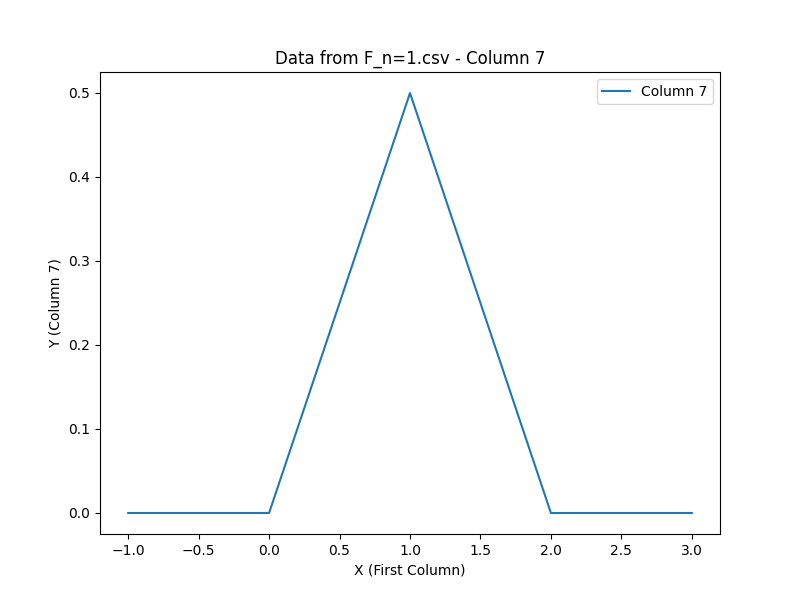
\includegraphics[width=\linewidth]{../figure/F_n=1.csv_Column_7.png} % 替换为你的图片路径
\end{minipage}
%%---------------------------------------------------------------------
$n=2$时,节点选择$0.0,\ 0.5,\  0.7,\  1.0$,结果如下\\
% 第一行:一张图片
\noindent % 确保左对齐
\begin{minipage}{0.3\textwidth}
	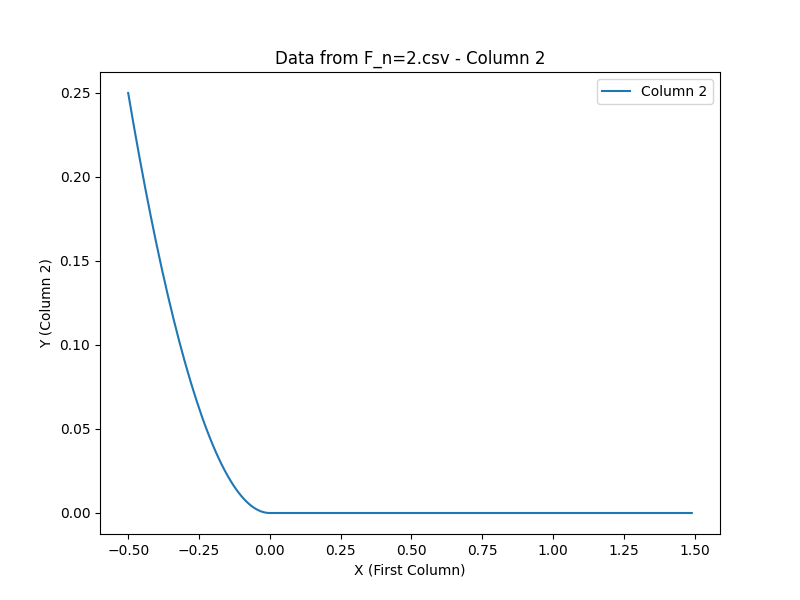
\includegraphics[width=4cm, height=4cm, keepaspectratio]{../figure/F_n=2.csv_Column_2.png} % 替换为你的图片路径
\end{minipage}

\vspace{0.5em} % 添加垂直间距

% 第二行:两张图片
\noindent % 确保左对齐
\begin{minipage}{0.3\textwidth}
	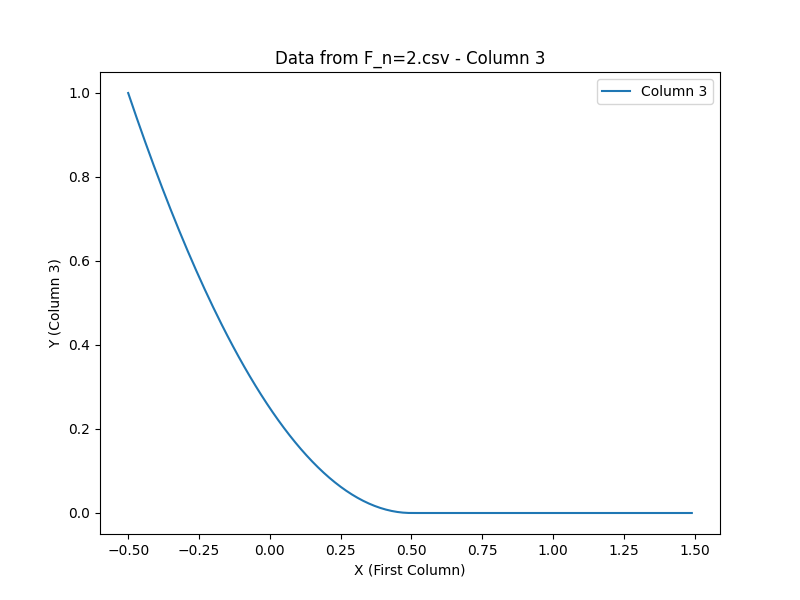
\includegraphics[width=4cm, height=4cm, keepaspectratio]{../figure/F_n=2.csv_Column_3.png} % 替换为你的图片路径
\end{minipage}
\hspace{0.5em} % 添加水平间距
\begin{minipage}{0.3\textwidth}
	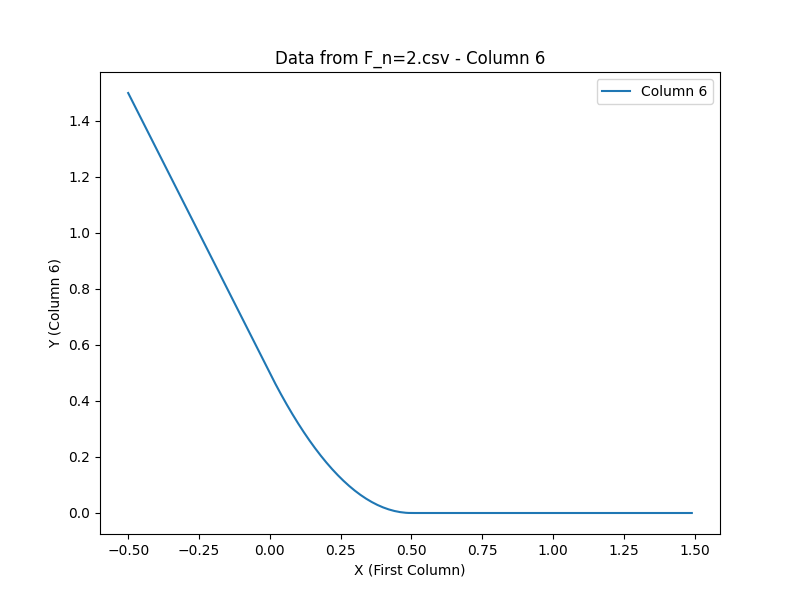
\includegraphics[width=4cm, height=4cm, keepaspectratio]{../figure/F_n=2.csv_Column_6.png} % 替换为你的图片路径
\end{minipage}

\vspace{0.5em} % 添加垂直间距

% 第三行:三张图片
\noindent % 确保左对齐
\begin{minipage}{0.3\textwidth}
	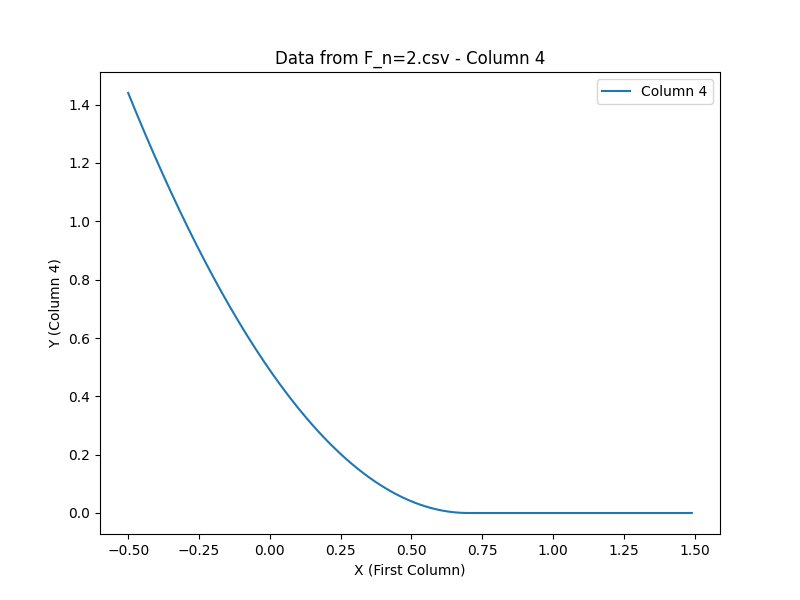
\includegraphics[width=4cm, height=4cm, keepaspectratio]{../figure/F_n=2.csv_Column_4.png} % 替换为你的图片路径
\end{minipage}
\hspace{0.5em} % 添加水平间距
\begin{minipage}{0.3\textwidth}
	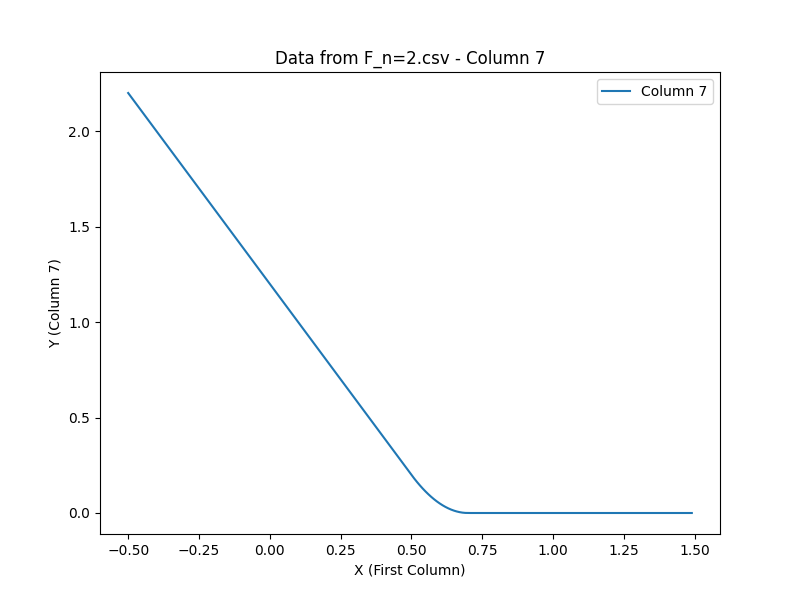
\includegraphics[width=4cm, height=4cm, keepaspectratio]{../figure/F_n=2.csv_Column_7.png} % 替换为你的图片路径
\end{minipage}
\hspace{0.5em} % 添加水平间距
\begin{minipage}{0.3\textwidth}
	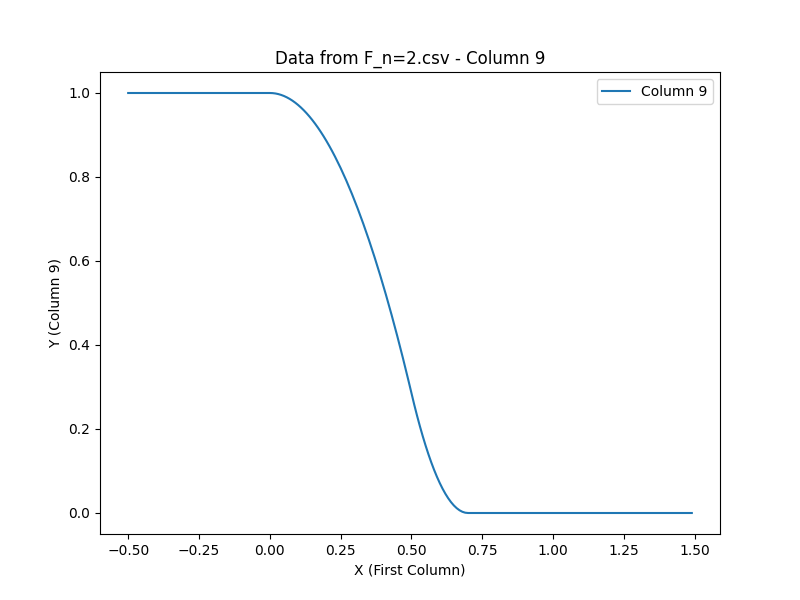
\includegraphics[width=4cm, height=4cm, keepaspectratio]{../figure/F_n=2.csv_Column_9.png} % 替换为你的图片路径
\end{minipage}

\vspace{0.5em} % 添加垂直间距

% 第四行:四张图片
\noindent % 确保左对齐
\begin{minipage}{0.23\textwidth}
	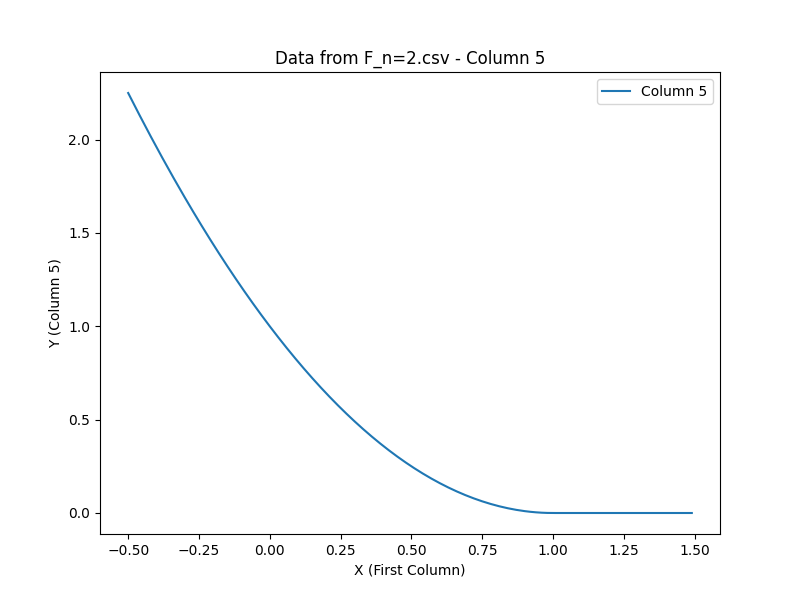
\includegraphics[width=4cm, height=4cm, keepaspectratio]{../figure/F_n=2.csv_Column_5.png} % 替换为你的图片路径
\end{minipage}
\hspace{0.5em} % 添加水平间距
\begin{minipage}{0.23\textwidth}
	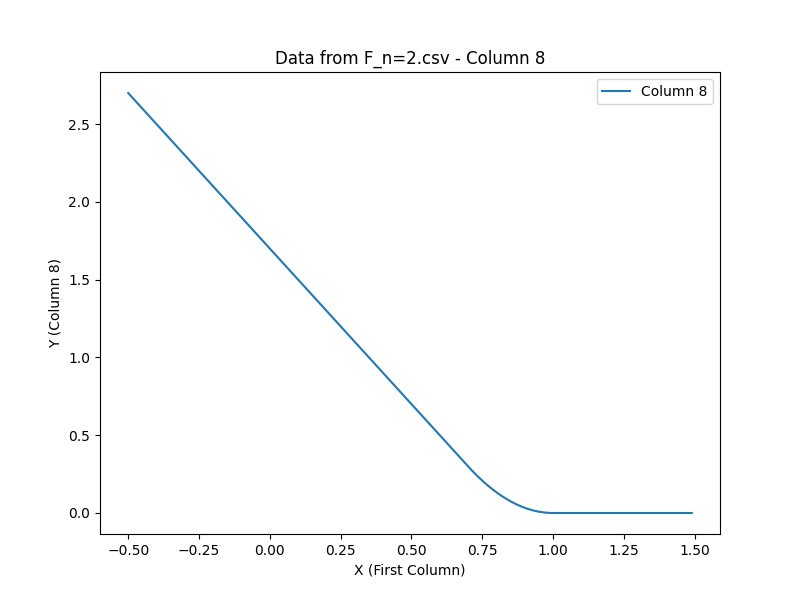
\includegraphics[width=4cm, height=4cm, keepaspectratio]{../figure/F_n=2.csv_Column_8.png} % 替换为你的图片路径
\end{minipage}
\hspace{0.5em} % 添加水平间距
\begin{minipage}{0.23\textwidth}
	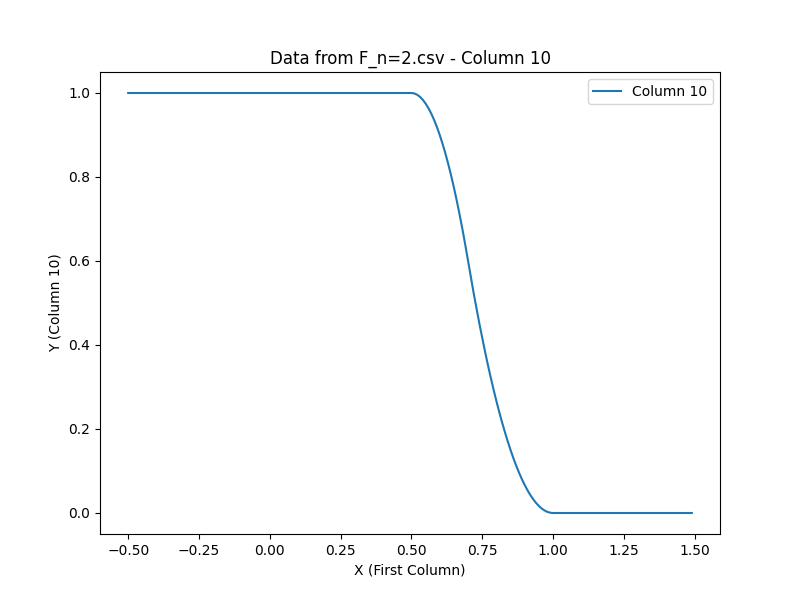
\includegraphics[width=4cm, height=4cm, keepaspectratio]{../figure/F_n=2.csv_Column_10.png} % 替换为你的图片路径
\end{minipage}
\hspace{0.5em} % 添加水平间距
\begin{minipage}{0.23\textwidth}
	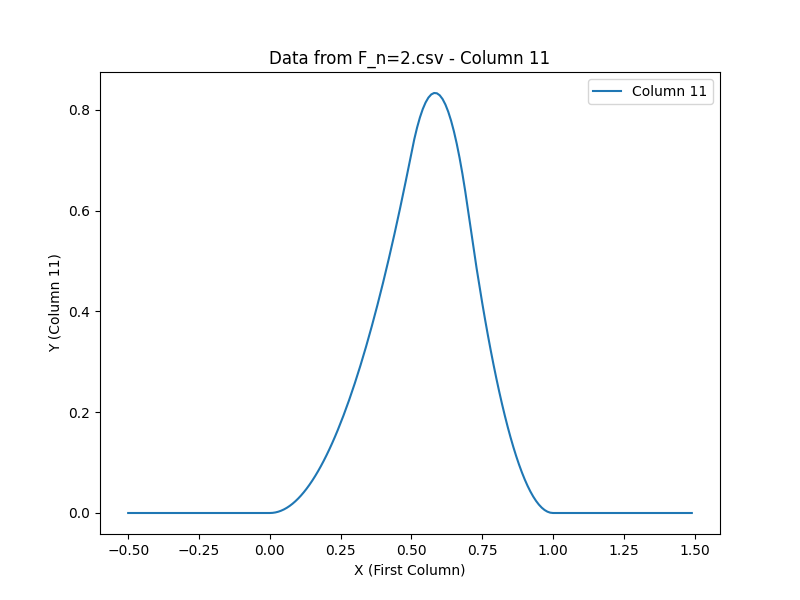
\includegraphics[width=4cm, height=4cm, keepaspectratio]{../figure/F_n=2.csv_Column_11.png} % 替换为你的图片路径
\end{minipage}

可以看到确实有$B_i^n(x) = (t_{i+n} − t_{i−1}) · [t_{i−1},..., t_{i+n}](t − x)^n_+$。而且通过提高差商的阶数,改善了一开始支集不是局部的问题。

\end{document}
